\chapter{Hurtownie danych}


Definicję Hurtowni Danych \ang{Data Warehouse}  przypisuje się Billowi Inmon'owi,
 który jako pierwszy opisał ją w 1992 roku.
Zgodnie z tą definicją hurtownią danych jest baza danych mającą następujące cztery cechy \cite{TodMan}.

\begin{itemize}
 \item Zorientowaną na temat \ang{ Subject-oriented} --- 
    dane są gromadzone 
    w~ściśle określony sposób, by możliwe było stworzenie czytelnego zestawienia danych.
   W hurtowni danych nie są przechowywane działania,
    czy operacje biznesowe.
   Hurtownia ograniczona się firmie do jednego działu 
    lub wybranego obszaru (np. biznesowego).
   Taka hurtownia jest określana jako lokalna hurtownia danych 
    lub tematyczna hurtownia danych \ang{data mart} stanowiąca podzbiór hurtowni danych.
 \item Nieulotność \ang{Non-volatile} --- 
    dane przechowywane w hurtowni danych nie są nigdy usuwane, ani modyfikowane. 
   Dane przeznaczone są wyłącznie do odczytu w celu utworzenia raportu na podstawie zadanego zapytania SQL.
 \item Integracja \ang{Intergrated} --- 
    w hurtowni danych znajdują się informacje, 
    przechowywanych przy wykorzystaniu dowolnych technologii. 
    W związku z faktem, że dane pochodzą z całej firmy, musi wystąpić ujednolicenie typów danych.
 \item Zmienność w czasie \ang{Time-Variant} --- musi zostać określone,
  co jaki okres czasu zostanie zapamiętany stan obecny w danej firmie.

\end{itemize}


\section{Powody budowania hurtowni danych.}
  
Uzasadnieniem budowania hurtowni danych może być:
\begin{itemize}
 \item \textbf{Przetwarzanie analityczne danych} \ang{On-Line Analytical Processing, OLAP} --  
    z danych zgromadzonych w hurtowni danych są tworzone zestawienia statystyczne,
    wykresy i~raporty w~różnych okresach czasowych.
 \item \textbf{Przeprowadzanie analizy danych bez ingerencji w operacyjną pracę systemów transakcyjnych} --
    analiza danych ze względu na bardzo dużą ich liczbę wymaga złożonych i czasochłonnych obliczeń.
    Dopuszczalne są zapytania kilkusekundowe, kilkuminutowe, mogą wystąpić nawet zapytania kilkudniowe. 
    Zapytania te jednak nie mogą wpływać na pracę systemu obsługującego klienta w czasie rzeczywistym,
    w którym takie zadanie musi zostać zrealizowane w możliwie jak najkrótszym czasie.
\item \textbf{Całościowy wgląd w dane firmy} --
    firmy bardzo często przechowują dane w różnych aplikacjach oraz na różnych środowiskach sprzętowych.
    Firma posiada głębszą wiedzę na temat zdarzeń, które miały miejsce w jej firmie,
    jeżeli ma możliwość zintegrowania danych. Na przykład osoba posiadająca sklep i warsztat samochodowy, 
    która chciałaby wiedzieć ile zostało sprzedanych części i~kto naprawiał samochód w jego warsztacie.
\item \textbf{Dostęp do danych historycznych} -- 
    dzięki danym historycznym możliwe jest wykonywanie analiz,
    z których można wyciągnąć wnioski, przekładające się na realne korzyści dla firmy.
\item \textbf{Ujednolicenie posiadanych informacji} -- 
   eliminuje tzw. problem wielu wersji prawdy firmy. 
   Raporty w frimie opierają się na danych pochodzących z różnych sektorów, które mogą generować zyski bądź straty.
   Firma w jednym obszarze może prosperować bardzo dobrze, zaś w innym może generować duże straty, które mogą w późniejszym czasie 
   stać się nawet przyczyną upadku tej firmy. Ujednolicenie informacji zebranych z różnych sektorów pozwoli na całościowy wgląd w
   obecny stan firmy.
\item \textbf{Wspomaganie decyzji} \ang{Decision Support, DS} -- wykonywanie 
  analizy symulującej scenariusz biznesowy.
\end{itemize}


\subsection{OLAP a OLTP}
Przetwarzanie analityczne danych \ang{On-Line Analytical Processing, OLAP} 
 i~przetwarzanie transakcyjne \ang{On-Line Transactional Processing,  OLTP}
 są to systemy optymalizowane pod kątem przetwarzania danych \cite{TodMan,Vincent_Rainardi}.

System OLTP jest przeznaczony dla pracowników, komunikujących się 
 z systemem bazodanowym w celu uzyskania określonych informacji 
 np. sprawdzenie dostępnych miejsc na danym koncercie.

Podstawowymi cechami systemów OLTP są:
\begin{enumerate}
 \item krótki czas realizacji bardzo dużej ilości zapytań, wykonywanych przez wielu użytkowników\label{OLTP_1},
 \item optymalizacja systemu bazodanowego pod kątem odczytu danych,
 \item częste usuwanie lub modyfikacja pojedynczych rekordów w bazie danych,
 \item aktualność danych przechowywanych w bazie.
\end{enumerate}

System OLAP jest przeznaczony dla pracowników przygotowujących zestawienie danych,
 raportów dla kadry zarządzającej,
 jak również dla analityków, 
 którzy na podstawie zadanych do hurtowni danych zapytań,
 mogą odkryć zależności występujące w firmie, a następnie wyciągnąć odpowiednie wnioski,
 które w ich opinii mogą dać firmie realny zysk.
 
Podstawowymi cechami systemów OLAP są:
\begin{enumerate}
 \item wykonywanie małej ilości zapytań przez niewielką liczbę użytkowników na dużym obszarze danych,
 \item cykliczne zasilane w ustalonych przedziałach czasowych,
 \item brak konieczności aktualizacji danych w bazie w czasie rzeczywistym.
\end{enumerate}


\subsection{Wspomaganie decyzji }
Systemy wspomagania decyzji \ang{decision support systems} tworzone są 
 w celu minimalizacji kosztów prowadzonej działalności,
 lepszego przewidywania ryzyka podejmowanych działań, podniesienia jakości w dziale obsługi klienta.
System OLAP jest 
 jednym z takich narzędzi, które wspierają podejmowanie decyzji.
Przykładowymi pytaniami, na które system powinien odpowiedzieć są \cite{TodMan}:
 \begin{enumerate}
  \item Jaki był dochód w rozbiciu na poszczególnych klientów?
  \item Jaki był procentowy wzrost lub spadek dochodu w porównaniu z zeszłym miesiącem?
  \item Jakie są cechy najlepszych/najgorszych klientów (cechy klientów muszą być ściśle określone)?
  \item Listę klientów, dla których współczynnik odejścia jest wysoki, a przynoszą oni zysk firmie.
 
 \end{enumerate}

Hurtownie danych odniosły sukces związany z zarządzaniem relacjami z klientem 
\ang{Customer Relationship Management, CRM},
 gdzie celem jest zatrzymanie najlepszych klientów oraz pozyskiwanie nowych,
 a także sprzedawanie im jak największej liczby produktów.
 

\section{Architektura hurtowni danych} \label{p_temat}
  W niniejszym podrozdziale zostanie przestawiona podstawowa architektura hurtowni danych oraz 
   proces związany z tworzeniem hurtowni, który jest bardzo drogi, czasochłonny, 
   a~żeby osiągnął sukces musi on być także ukierunkowany na klienta,
   czyli dostosowany do jego wymagań, 
   które opierają się głównie na intuicji.
   Na rysunku \ref{fig:AHD} przedstawione zostały główne elementy hurtowni danych oraz kierunek przepływu danych.
   Strzałki pokazują kierunek przepływu danych \cite{TodMan,link_hd}.

\begin{center}
\begin{figure}[H]
  \begin{center}
    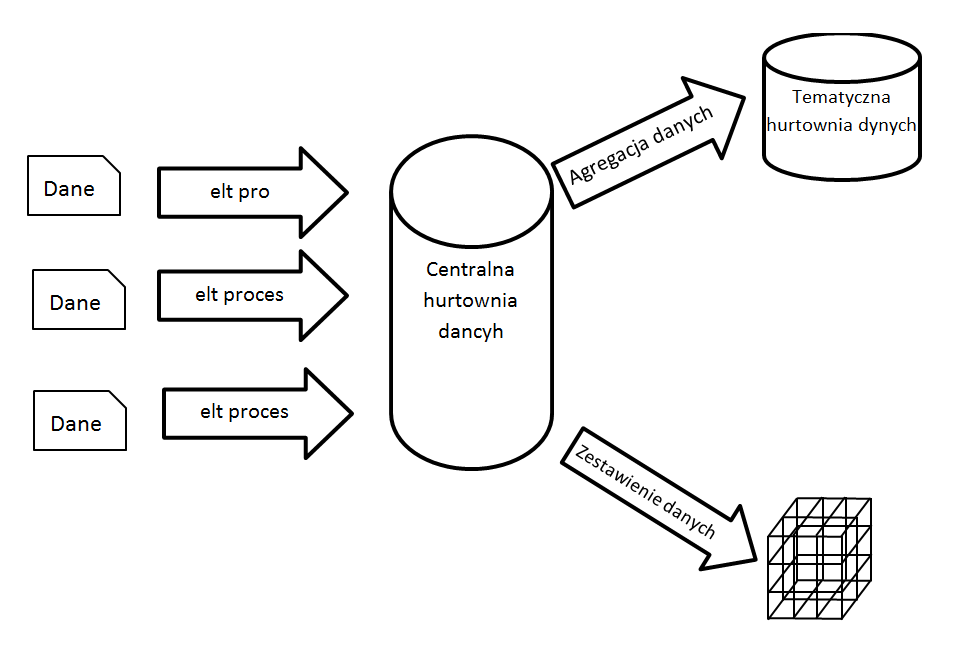
\includegraphics[width=0.7\textwidth]{AHD.png}
  \end{center}
 \caption{Architektura hurtowni danych. }
    \label{fig:AHD}
\end{figure}
\end{center}


Strukturę przepływu danych możemy podzielić na:
\begin{itemize}
 \item \textbf{Źródło danych \ang{source} } --- 
    są to dane, które będą pobierane do hurtowni danych. 
 \item \textbf{Proces ETL \ang{extract, transfer, load} } --- 
    procesem ETL nazywamy czynności wykonywane w celu pobrania danych źródłowych,
    przekształcenie danych na odpowiedni format, a następnie umieszczenie ich w centralnej hurtowni danych.
    Proces ETL zostanie dokładnie omówiony w rozdziale drugim.
 \item \textbf{Centralna hurtownia danych \ang{center data  warehouse}} --- 
    jest to miejsce docelowe przetworzonych danych ze źródeł,						                                          
 \item \textbf{hurtownie tematyczne \ang{data marts}} --- 
    zawierają wybrane dane z centralnej hurtowni danych w~sposób 
    zagregowany, umożliwiające szybkie operowanie sporządzanie raportów,
 \item \textbf{zestawienie danych } --- 
    docelowym produktem hurtowni danych jest tworzenie odpowiednich zestawień danych.
    Na rysunku \ref{fig:AHD}, został przedstawiona jako kostka.
\end{itemize}

 
Tworzenie hurtowni danych jest stosunkowo młodą dziedziną, która się dynamicznie rozwija.
Dzięki zastosowaniom CRM hurtownie danych odniosły znaczący sukces, co spowodowało większe zapotrzebowanie na przechowywanie i~analizowanie danych historycznych. 
Przedstawiona architektura danych na rysunku \ref{fig:AHD}, nie spełnia swojej roli jako hurtowni danych, w których przyrost danych jest bardzo duży.
Poniżej została przedstawiona inna architektura danych.
\begin{center}
\begin{figure}[H]
  \begin{center}
    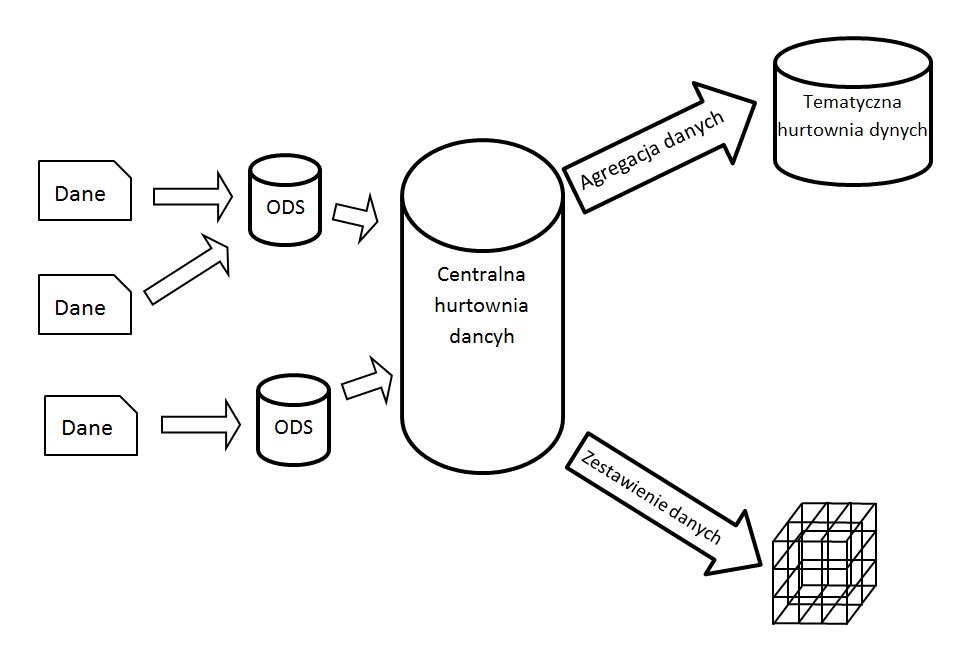
\includegraphics[width=0.7\textwidth]{AHD_ODS.png}
  \end{center}
  \caption{Architektura hurtowni danych z magazynem danych ODS. }
    \label{fig:ODS}
\end{figure}
\end{center}

Do architektury z rysunku \ref{fig:AHD} został dodany magazyn danych operacyjnych \ang{operational data store, ODS}, który
pełni role magazynu danych. Ładowane są do niego dane pobrane ze źródeł i przetworzone w celu uzyskania zgodności typów danych.
Kolejnym etapem jest załadowanie danych w sposób zagregowany do centralnej hurtowni danych.


\section{Projektowanie hurtowni danych.}
Projektowanie hurtowni danych tak jak relacyjnych baz danych polega na utworzeniu następujących modeli \cite{TodMan}:

\begin{itemize}
 \item \textbf{Model pojęciowy} --- 
    przy użyciu języka biznesowego w danej firmie opisuje się cele biznesowe, 
    które będzie można określić przez zgromadzenie ściśle określonych danych.
   Na modelu pojęciowym powinny, być zaznaczone nazwy kolumn, które mają być przechowywane 
    w tabeli znajdującej się w hurtowni danych
 \item \textbf{Model logiczny} --- 
    jest to opis elementów  logicznych hurtowni danych, wykonany np. w języku UML.
 \item \textbf{Model fizyczny} --- 
    jest to opis indeksowania, partycjonowania, opis sprzętu komputerowego, sieci
     rozmieszczenia poszczególnych zasobów fizycznych.
\end{itemize}

Najpopularniejszymi metodami przyjętymi podczas tworzenia hurtowni danych są:
\begin{itemize}
 \item \textbf{Projektowanie wstępujące} (od szczegółu do ogółu)---
    polega na tworzeniu wszystkich etapów hurtowni danych
    jednocześnie, a następnie na integracji poszczególnych etapów ze sobą.
 \item \textbf{Projektowanie zstępujące} ---
    dopóki jeden etap tworzenia hurtowni danych się nie skończy, 
    następny nie może się rozpocząć.
    Jeżeli pojawią się błędy to wraca się do poprzedniego etapu i zaczyna się prace 
     na kolejnym etapie od nowa.
\end{itemize}



\section{Wielowymiarowy model danych}
Wielowymiarowym modelem danych \ang{Multidimensional Data Model} 
nazywamy dane zorganizowane w:
\begin{itemize}
 \item \textbf{Fakt \ang{facts}  } --- 
    są to dane opisujące jakieś zdarzenie. Tabelę przechowującą te dane nazywamy \textit{tablicą faktów}.
   Fakt opisywany jest przez wymiary i miary.
 \item \textbf{Wymiar \ang{dimension}} --- 
    jest jakąś cechą opisującą dany fakt. Cechy te znajdują się w tablicy wymiarów i są opisywane przez atrybuty.
 \item \textbf{Atrybut} \ang{ attribute}  --- 
    przechowuje dodatkowe informacje na temat wymiaru.
 \item \textbf{Miara \ang{measures}} --- 
    jest wartością mierzalną, przypisaną do pojedynczego rekordu w tablicy faktów. 
\end{itemize}

Model ten jest zintegrowaną częścią systemu OLAP.
Podstawowym atutem wielowymiarowego modelu danych jest proste zrozumienie hurtowni danych 
 i poruszania się po niej w sposób efektywny, szybsze wykonywanie zapytań zadawanych do hurtowni danych. 
Jak również możliwość analizy danych w różnych wymiarach, 
które jest bardzo istotne ze względów biznesowych:
\begin{itemize}
 \item Oglądanie informacji rozłożonych w czasie,
 \item Wyświetlanie informacji w sposób graficzny,
 \item Możliwość zmiany przekroju danych w dowolny sposób,
 \item Analizę danych pod kątem informacji istotnych dla danej firmy.
\end{itemize}

Podstawowymi schematami wielowymiarowego modelu danych są:
\begin{itemize}
 \item schemat gwiazdy \ang{Star schema} 
 \item schemat płatka śniegu \ang{Snowflake schema}
\end{itemize}

\subsection{Schemat gwiazdy}
Schemat gwiazdy jest podstawowym schematem wielowymiarowego modelu danych,
 w którym znajduje się jedna tabela faktów połączona z wieloma tabelami wymiarów.
Tabela faktów w powyższym schemacie jest w trzeciej postaci normalnej, a tabela wymiarów jest w drugiej postaci normalnej.
Dzięki takiej strukturze możliwe jest szybsze przeglądanie danych poprzez \cite{TodMan, link_hd}:
\begin{itemize}
 \item poszczególne wymiary,
 \item sumowanie danych,
 \item agregację danych,
 \item filtrowanie danych
\end{itemize}

Na rysunku  \ref{fig:gwiazda} został przedstawiona przykładowa architektura schematu gwiazdy.
\begin{center}
\begin{figure}[H]
  \begin{center}
    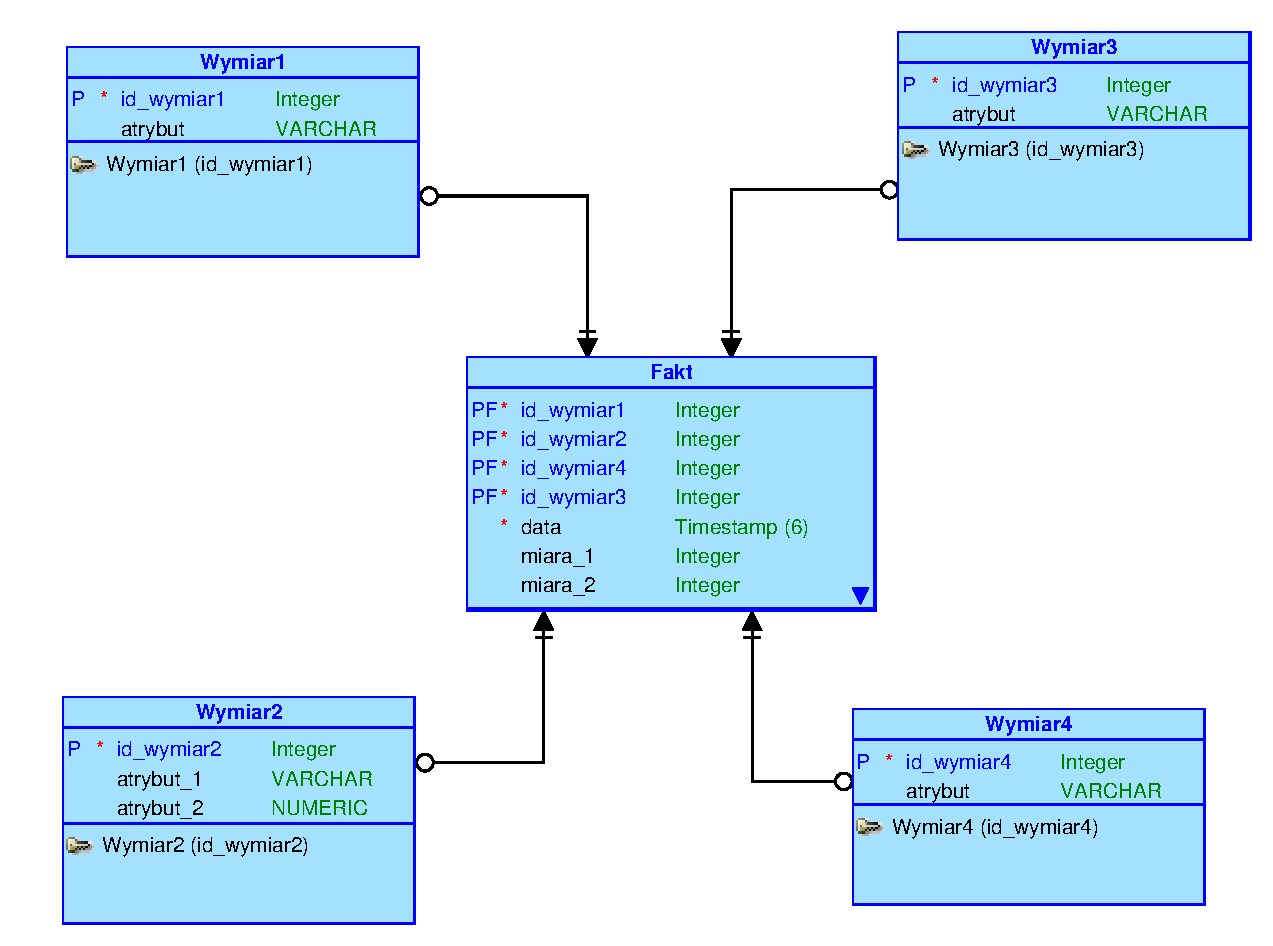
\includegraphics[width=0.7\textwidth]{gwiazda.pdf}
  \end{center}
  \caption{Przykładowy schemat gwiazdy w postaci abstrakcyjnej. }
    \label{fig:gwiazda}
\end{figure}
\end{center}
Poniżej znajduje się listing zapytań do bazy danych w języku PostgreSQL,
 który realizuje model logiczny gwiazdy zawarty na rysunku \ref{fig:gwiazda}
\lstinputlisting[language=sql, caption = {Listing kodu tworzący schemat gwiazdy. } ]{"./sql/gwiazda.sql"}

\subsection{Schemat płatka śniegu}
Architektura schematu gwiazdy jest uproszczoną formą architektury płatka śniegu.
Podstawową różnicą pomiędzy tymi schematami jest tabela wymiarów, która jest znormalizowana.

Schemat płatka śniegu jest stosowany wtedy, gdy tabela wymiarów osiąga duży rozmiar.
Normalizuje się tabele wymiarów, aby zmniejszyć jej liczebność, dzięki czemu czas zapytań, 
powinien się znacząco skrócić. 
Wadą tego podejścia jest, że im bardziej znormalizowana jest tabela wymiarów,  
 tym bardziej skomplikowane łączenia SQL muszę zostać użyte, aby pobrać odpowiednie
dane z hurtowni danych. \cite{TodMan, cube}

Przykładowa architektura płatka śniegu został przedstawiona na rysunku \ref{fig:platek_sniegu} .

\begin{center}
\begin{figure}[H]
  \begin{center}
    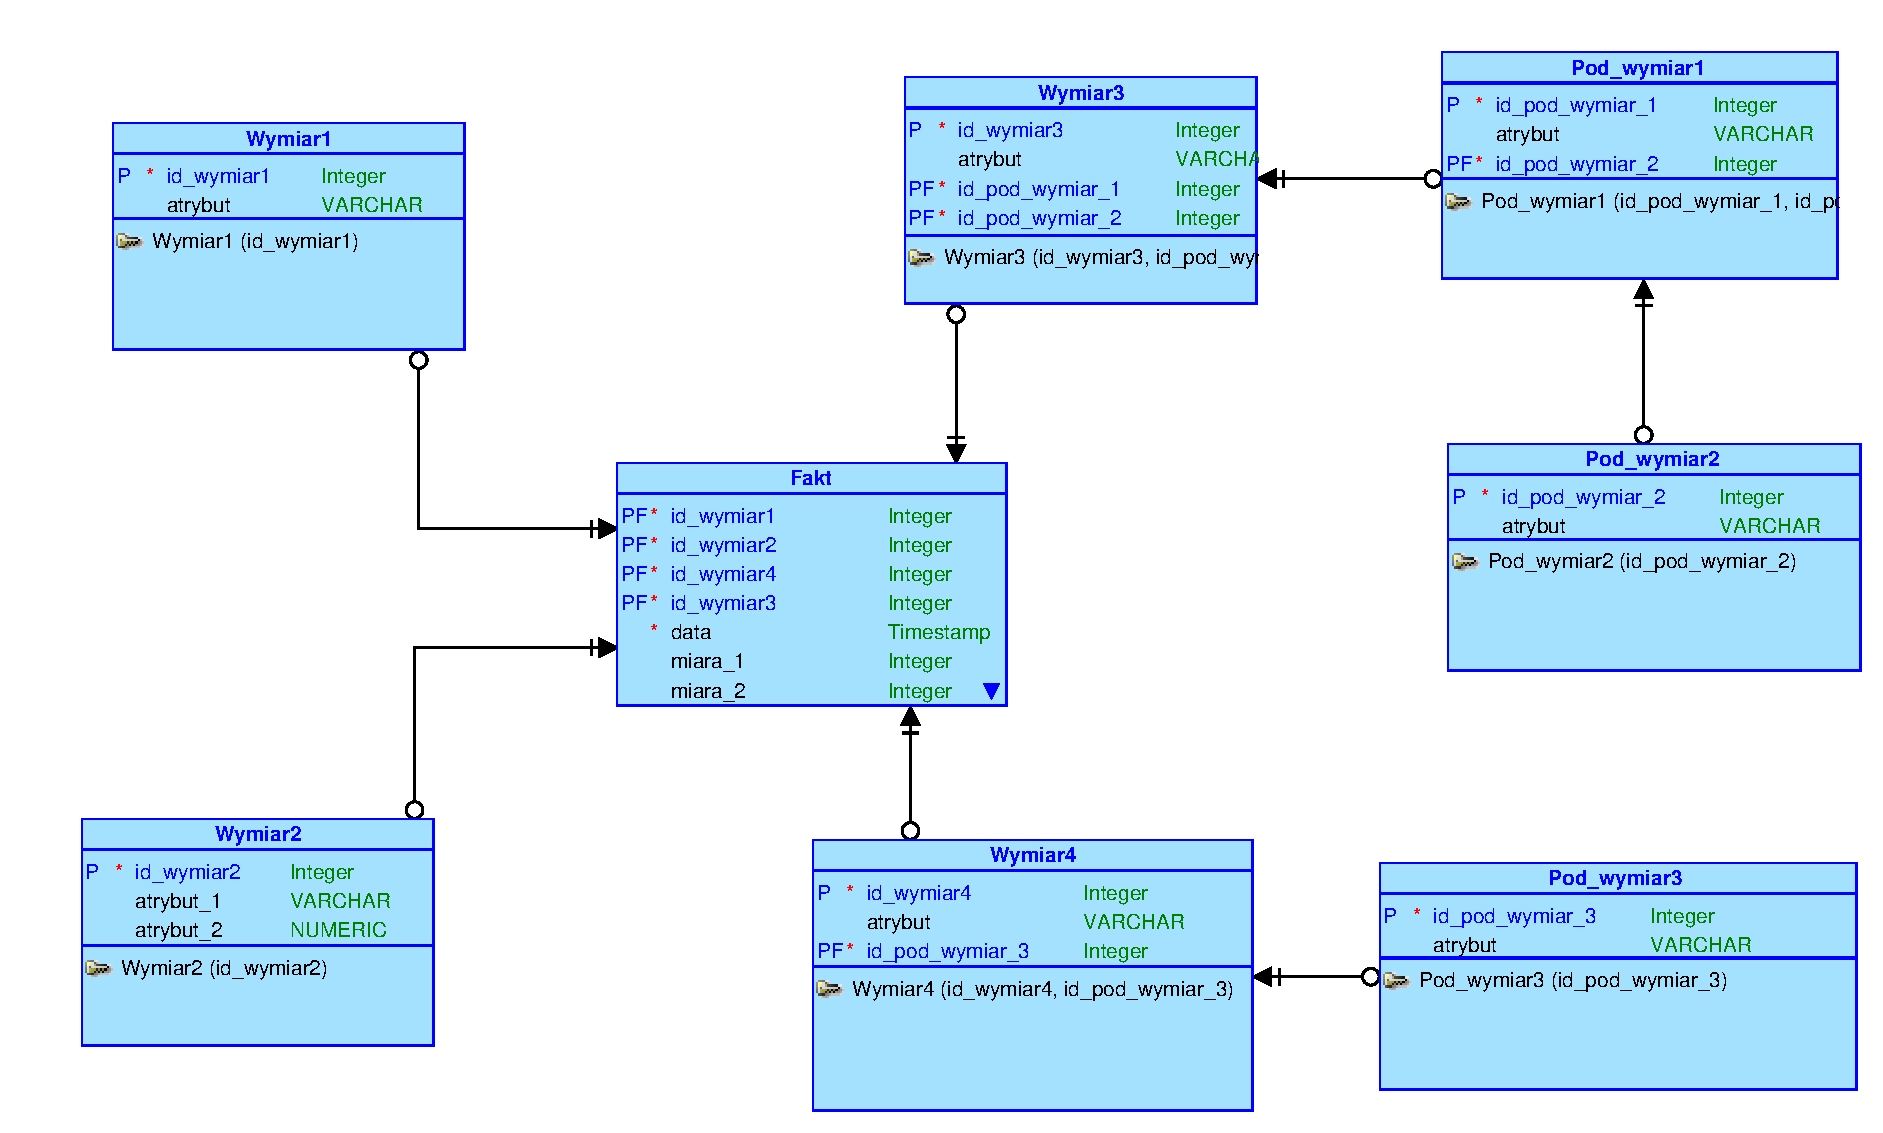
\includegraphics[width=0.7\textwidth]{platek_sniegu.pdf}
  \end{center}
  \caption{Przykładowy schemat płatka śniegu w postaci abstrakcyjnej. }
    \label{fig:platek_sniegu}
\end{figure}
\end{center}







\begin{comment}
 
\end{comment}
